\documentclass[tikz,border=2pt]{standalone}
\usepackage{amsmath,amssymb}
\usepackage{tikz}
\usetikzlibrary{arrows.meta}

\begin{document}
% An artificial variable R gives a >= or = row a starting basic variable (coefficient +1);
% it is a temporary crutch that must be driven back to zero before the real LP is solved.
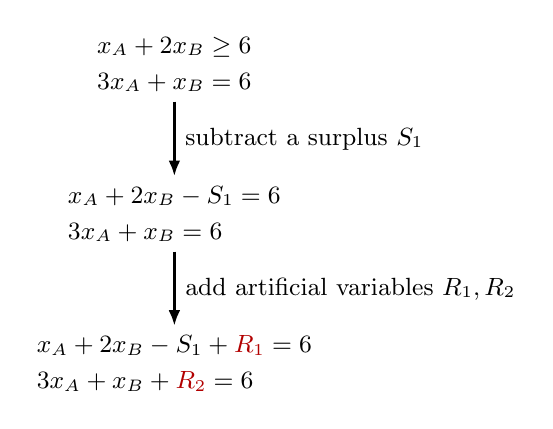
\begin{tikzpicture}[every node/.style={font=\small}, >={Latex[length=2mm]}]
	\node[align=left] (a) at (0,0) {$x_A+2x_B\ge6$\\[2pt] $3x_A+x_B=6$};
	\node[align=left] (b) at (0,-1.9) {$x_A+2x_B-S_1=6$\\[2pt] $3x_A+x_B=6$};
	\node[align=left] (c) at (0,-3.8) {$x_A+2x_B-S_1+\textcolor{red!70!black}{R_1}=6$\\[2pt] $3x_A+x_B+\textcolor{red!70!black}{R_2}=6$};
	\draw[->, very thick] (a) -- (b) node[midway, right] {subtract a surplus $S_1$};
	\draw[->, very thick] (b) -- (c) node[midway, right] {add artificial variables $R_1,R_2$};
	\end{tikzpicture}
\end{document}
